\section{Desarrollo en Laboratorio}

En esta sección se documenta la implementación física de la red RC de segundo orden. El diseño se abordó mediante un proceso de escalamiento con $k_m<1$, partiendo de una red de alta impedancia para obtener configuraciones de menor magnitud óhmica, validando la flexibilidad de las ecuaciones de escalamiento.

\subsection{Planteamiento del Circuito Original}

El circuito base se construyó utilizando componentes de alta impedancia para establecer la referencia de operación. Los parámetros definidos para el prototipo original fueron:

\begin{itemize}
	\item $R_1 = R_2 = 10\,\text{k}\Omega$.
	\item $C_1 = C_2 = 10\,\text{nF}$.
\end{itemize}
La señal de entrada se fijó en $1.71\,\text{V}_{\text{rms}}$ con una frecuencia de operación de $1\,\text{kHz}$.

\begin{center}
	\begin{circuitikz}[american]
		\draw (0,0) to[vsourcesin, l=$1.71\,\text{V}_{\text{rms}}$, f=$1\,\text{kHz}$] (0,3)
		(0,3) to[R, l=$R_1(10\,\text{k}\Omega)$] (3,3)
		(3,3) to[C, l=$C_1(10\,\text{nF})$] (3,0)
		(3,3) to[R, l=$R_2(10\,\text{k}\Omega)$] (6,3)
		(6,3) to[C, l=$C_2(10\,\text{nF})$] (6,0)
		(0,0) -- (6,0)
		(0,0) node[ground] {};
	\end{circuitikz}
\end{center}

\begin{figure}[H]
	\centering
	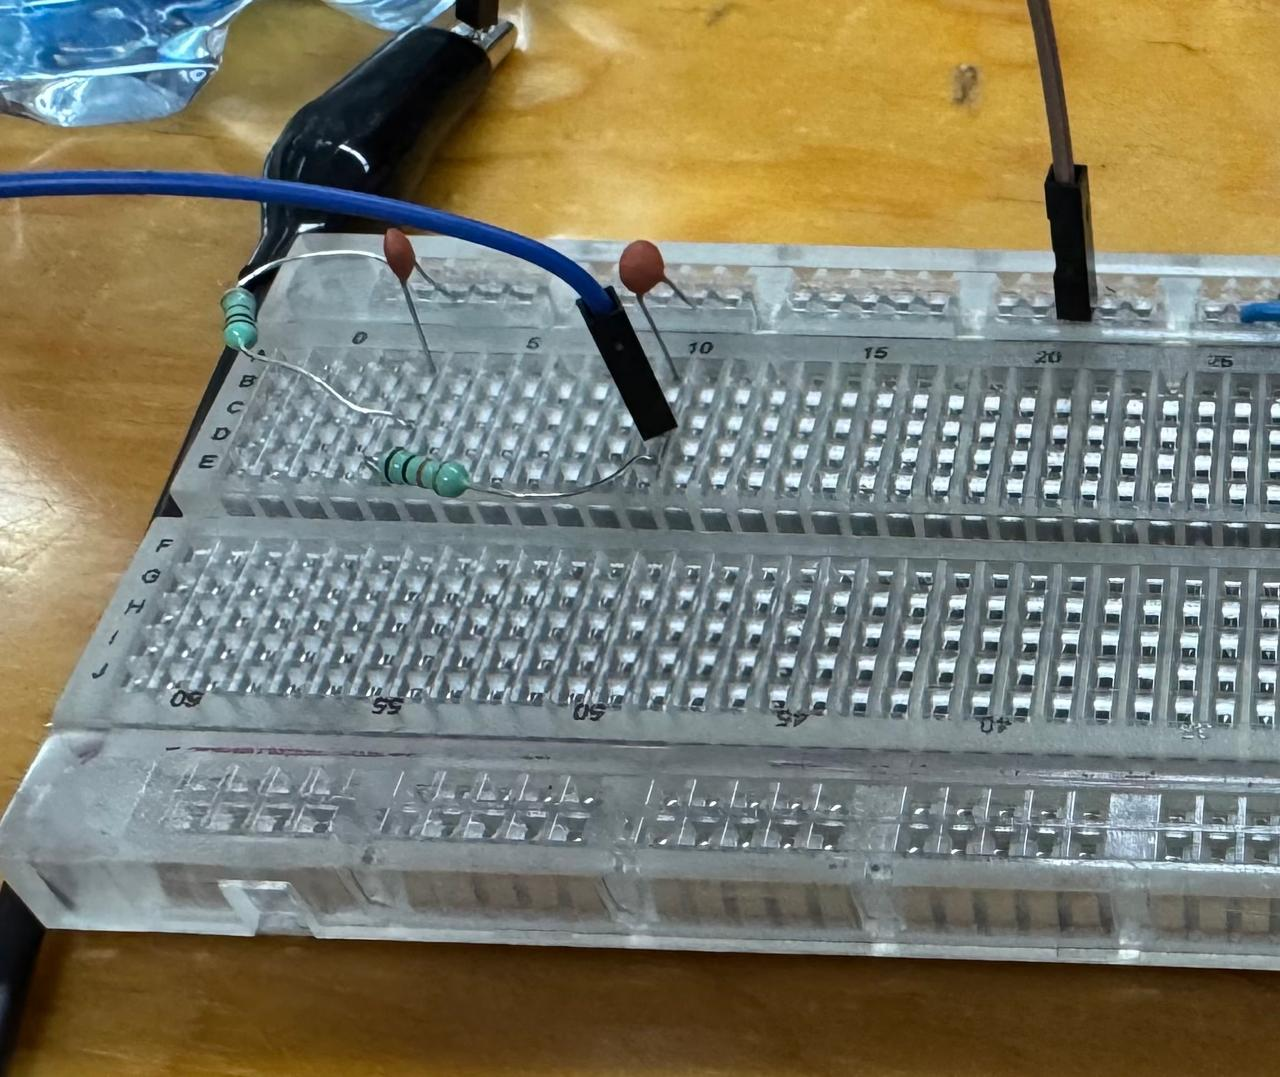
\includegraphics[width=0.6\linewidth]{assets/img/circuito_original.jpeg}
	\caption{Implementación del circuito prototipo original ($10\,\text{k}\Omega, 10\,\text{nF}$).}
\end{figure}

\subsection{Escalamiento de Impedancia ($K_m = 0.1$)}
Se aplicó un factor de magnitud $K_m = 0.1$ con el objetivo de reducir la impedancia total de la red por un factor de diez. Este procedimiento permite manejar corrientes más elevadas en la red manteniendo la respuesta en frecuencia inalterada.

\subsubsection{Cálculo de Componentes Escalados}
\begin{itemize}
	\item $R' = R \cdot K_m = 10\,\text{k}\Omega \cdot 0.1 = 1\,\text{k}\Omega$.
	\item $C' = \frac{C}{K_m} = \frac{10\,\text{nF}}{0.1} = 0.1\,\mu\text{F}$.
\end{itemize}

\begin{center}
	\begin{circuitikz}[american]
		\draw (0,0) to[vsourcesin, l=$1.71\,\text{V}_{\text{rms}}$, f=$1\,\text{kHz}$] (0,3)
		(0,3) to[R, l=$R_1'(1\,\text{k}\Omega)$] (3,3)
		(3,3) to[C, l=$C_1'(0.1\,\mu\text{F})$] (3,0)
		(3,3) to[R, l=$R_2'(1\,\text{k}\Omega)$] (6,3)
		(6,3) to[C, l=$C_2'(0.1\,\mu\text{F})$] (6,0)
		(0,0) -- (6,0)
		(0,0) node[ground] {};
	\end{circuitikz}
\end{center}

\begin{figure}[H]
	\centering
	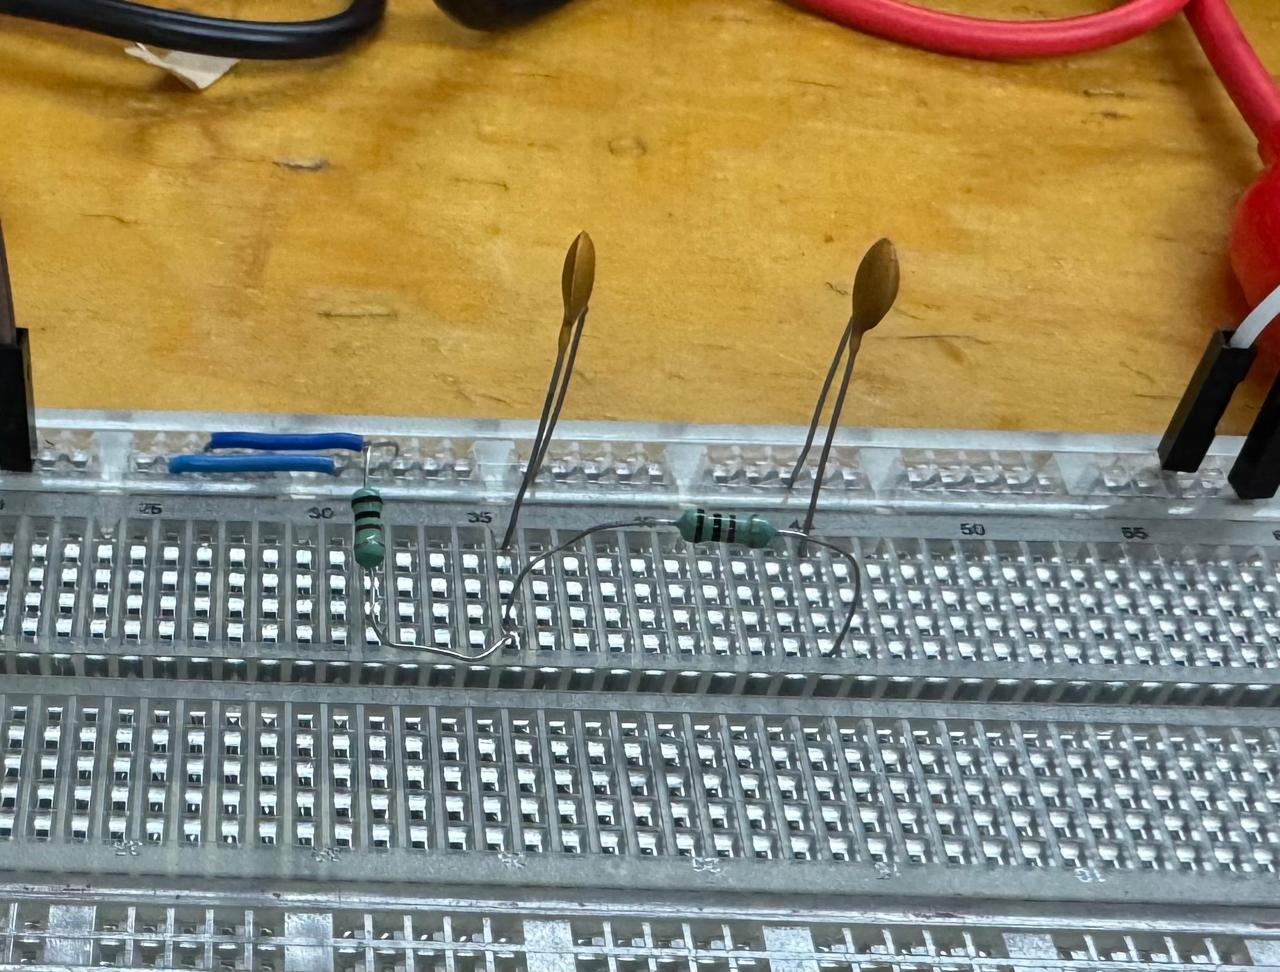
\includegraphics[width=0.8\linewidth]{assets/img/circuito_escImp.jpeg}
	\caption{Circuito con escalamiento de magnitud fraccional ($K_m = 0.1$).}
\end{figure}

\begin{figure}[H]
	\centering
	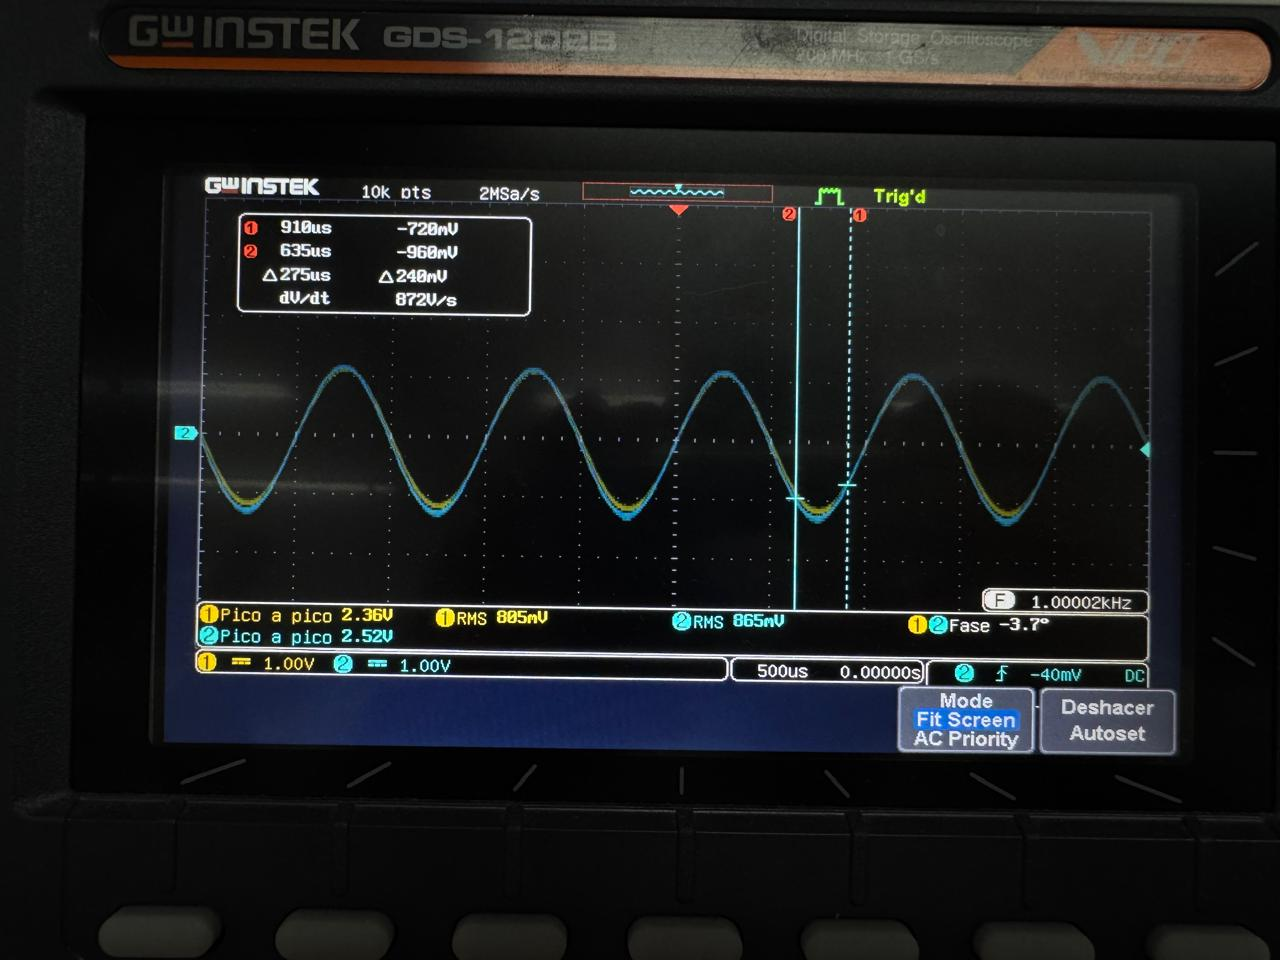
\includegraphics[width=0.8\linewidth]{assets/img/osc_ogimp.jpeg}
	\caption{Respuesta del escalamiento de impedancia en el osciloscopio. Azul(original) - amarillo(escalado) .}
\end{figure}

\subsection{Escalamiento en Frecuencia ($K_f = 0.5$)}
Para la última etapa, se buscó desplazar la respuesta del filtro hacia frecuencias más bajas..

Partiendo del diseño original ($10\,\text{k}\Omega, 10\,\text{nF}$), aplicamos el escalamiento de frecuencia con $K_f = 0.5$:

\begin{equation}
	C' = \frac{C}{K_f} \implies C'= \frac{10\text{nF}}{0.5} \implies C' = 20\text{nF}
\end{equation}

\begin{equation}
	R' = R
\end{equation}


Este factor indica que la frecuencia de operación se desplazó a la mitad de su valor, manteniendo el nivel de impedancia de $10\,\text{k}\Omega$.

\begin{center}
	\begin{circuitikz}[american]
		\draw (0,0) to[vsourcesin, l=$1.71\,\text{V}_{\text{rms}}$, f=$500\,\text{Hz}$] (0,3)
		(0,3) to[R, l=$R_1'(10\,\text{k}\Omega)$] (3,3)
		(3,3) to[C, l=$C_1'(20\,\text{nF})$] (3,0)
		(3,3) to[R, l=$R_2'(10\,\text{k}\Omega)$] (6,3)
		(6,3) to[C, l=$C_2'(20\,\text{nF})$] (6,0)
		(0,0) -- (6,0)
		(0,0) node[ground] {};
	\end{circuitikz}
\end{center}

\begin{figure}[H]
	\centering
	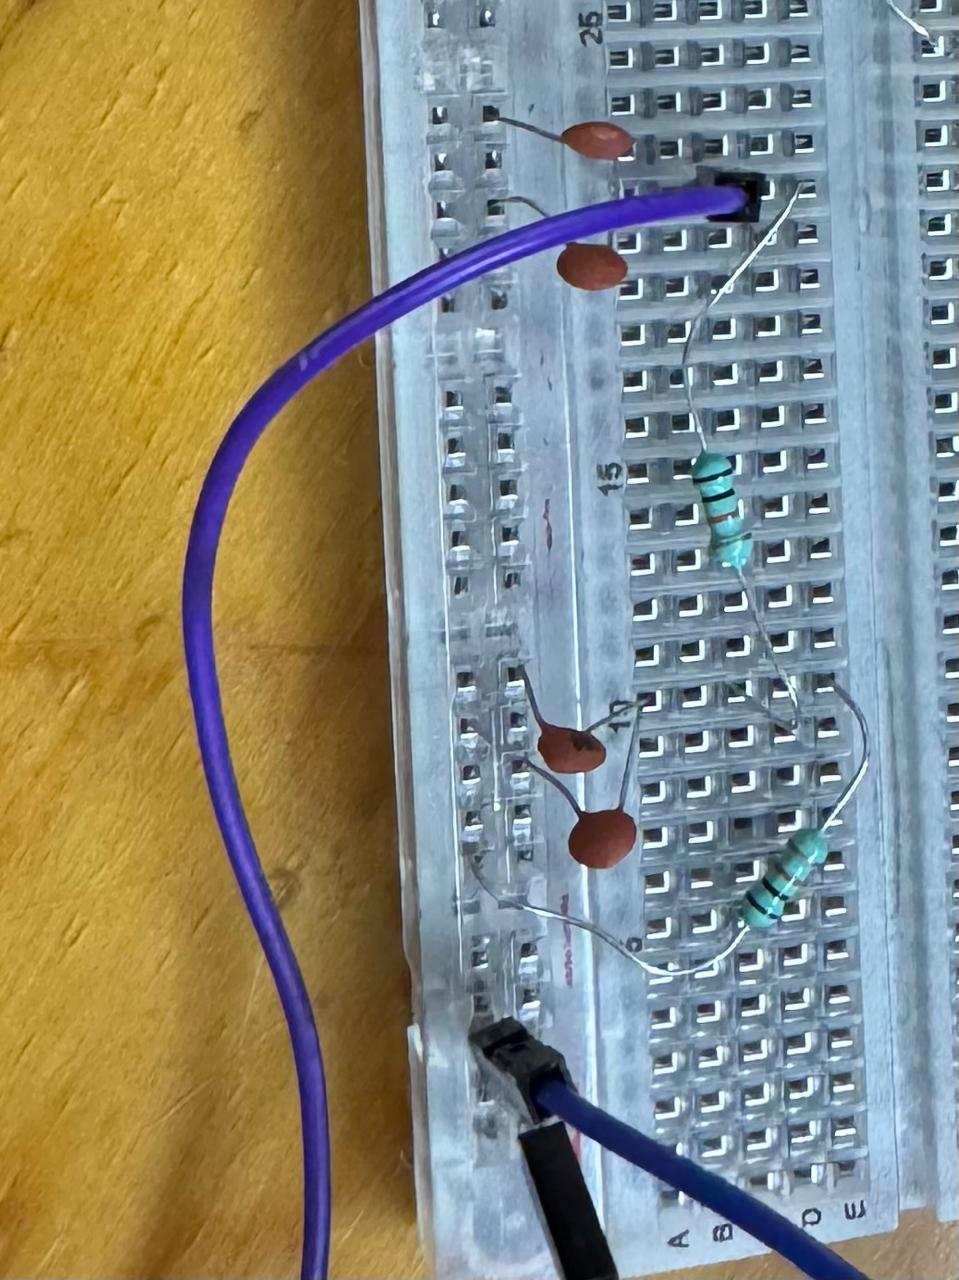
\includegraphics[width=0.8\linewidth]{assets/img/circuito_escfrec.jpeg}
	\caption{Circuito con escalamiento en frecuencia ($K_f = 0.5$).}
\end{figure}

\begin{figure}[H]
	\centering
	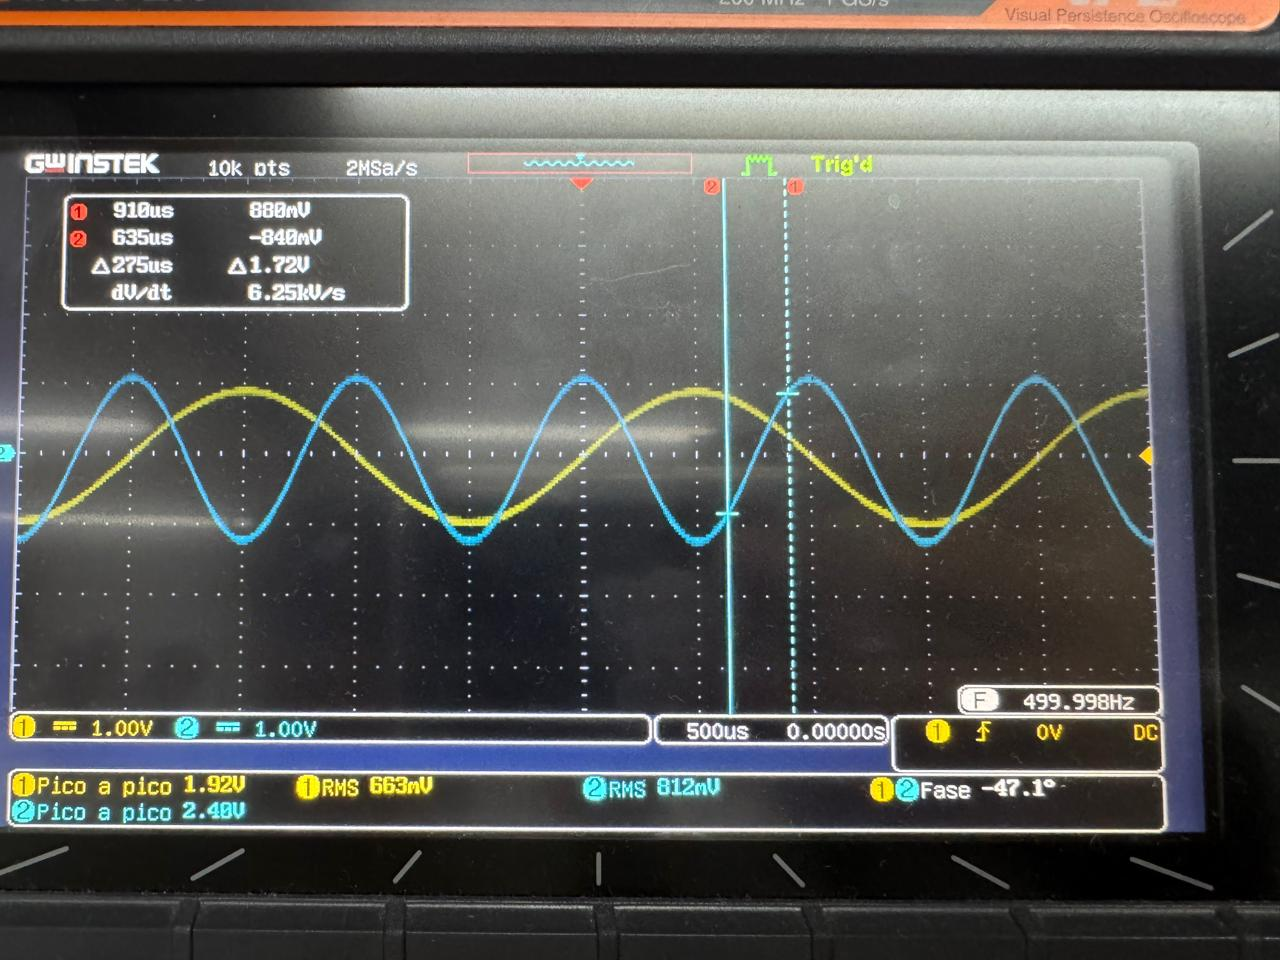
\includegraphics[width=0.8\linewidth]{assets/img/osc_ogfrec.jpeg}
	\caption{Respuesta del escalamiento en frecuencia en el osciloscopio. Azul(original) - amarillo(escalado).}
\end{figure}